\RequirePackage{luatex85,shellesc}
\documentclass[]{resonance}
\usepackage{pgf,tikz}
\usepackage{tikzsymbols}
\usepackage[breakable]{tcolorbox}
\usepackage{nameref}
\usepackage{pgfplots}
\usepackage{grffile}
\usepackage{amsmath}
\usepackage{sidecap}
\usepackage{mathtools}
\usepackage{wrapfig}
\usepackage{chemfig}
\usepackage{siunitx}
\usepackage{todonotes}
\usepackage{tabularx} 
\usepackage{amssymb}
\usetikzlibrary{shapes,backgrounds,calc,arrows,arrows.meta}
\pgfplotsset{compat=1.15}

\usepackage[acronym]{glossaries}
%\newglossaryentry{CaM}
%{
%    name=Calmodulin,
%    description={Calmodulin}
%}

\newacronym{camkii}{CaMKII}{calcium/calmodulin dependant protein Kinase II}
\newacronym{cam}{CaM}{calmodulin}
\newacronym{psd}{PSD}{Post Synaptic Densitiy}
\newacronym{ca}{Ca\textsuperscript{++}}{calcium}
\newacronym{pp1}{PP1}{protein phophatase 1}
\newacronym{pp2}{PP2}{protein phophatase 2}
\newacronym{cacam}{Ca\textsuperscript{++}/CaM}{calcium/calmodulin complex}
\newacronym{i1p}{I1P}{phosphorylated inhibitor-1}
\newacronym{i1ppp1}{I1P.PP1}{I1P-PP1 complex}
\newacronym{i1}{I1}{inhibitor-1}
\newacronym{can}{CaN}{calcineurin}
\newacronym{pka}{PKA}{protein kinase A}
\newacronym{darpp}{DARPP-32}{a dopamine- and cyclic-AMP regulated neuronal phosphoprotein}
\newacronym{i2}{I2}{inhibitor 2}
\newacronym{sbgn}{SBGN}{System Biology Graphical Notation}
\newacronym{ltp}{LTP}{Long Term Potentiation}
\newacronym{ltd}{LTD}{Long Term Depression}
\newacronym{nmda}{NMDA}{N-methyl-D-asparate}
\newacronym{nmdar}{NMDAR}{N-methyl-D-asparate receptor}
\newacronym{ampa}{AMPA}{$\alpha$-amino-3-hydroxy-5-methyl-4-isoxazolepropionic acid}
\newacronym{mz}{MZ}{Miller and Zhabotinksy}


\newcommand\Fig[1]{\textit{Figure~\ref{#1}}}
\newcommand\TT[1]{\texttt{#1}}

% Title Page
\title{Switches in the brain?} 
\secondTitle{A potential mechanism for long-term memory storage}
\author{Dilawar Singh}
\date{\today}
\begin{document}
\maketitle

% Author info here
\authorIntro{
    
\includegraphics[width=2cm]{./dilawar.jpg}\\
    Dilawar Singh is currently a graduate student at National Center for
    Biological Sciences (NCBS), Bengaluru. His hobby is to convince people to
    move to open-source softwares to live happily ever after.
}


\begin{abstract}

    We forget often. But we remember some memories as long as we live.
    This means that our brain is capable of protecting memories for years.
    This is a remarkable feat given that the \emph{biochemical hardware}
    involved in creating new memories is a hostile place for
    its storage.  What are the challenges involved? And what type of 
    biochemical mechanisms may overcome them? This article explores a major
    hypothesis that molecular switches may be behind our remarkable ability to
    remember for a lifetime.

\end{abstract}

\maketitle
\monthyear{May 2018}
\artNature{GENERAL ARTICLE}

\section{Introduction}\label{sec:intro}

Our brain is made up of roughly 100 billion neurons, joined together with over
100 trillion connections called \textbf{synpase}s. Each neuron on average makes
1000 connections. It is now widely accepted that memories are created by
changing these connections. 

Let's label these synapses as $s_1, s_2, \ldots s_n$. During memory formation, a
subset of these synapses will undergo changes. For example, my memory of being
chased by a ferocious street dog named \emph{Lalu} (lets call it
$M_\text{Lalu}$) is stored in the set of synapses $M_\text{Lalu}=(s_{10},
s_{21}, s_{12},\ldots,s_{331})$ i.e., these connections were changed during my
troubling encounter with Lalu. I sometimes recall this memory whenever I see a
similar looking dog.

\begin{figure}[!b] 
    \caption{Memory formation and forgetting in brain. During formation of
        a memory, some synapses become stronger (larger black dots). 
        The longer you can maintain these connections, the longer you 
        can hold on to this memory.
    }
    \label{fig:engram}
    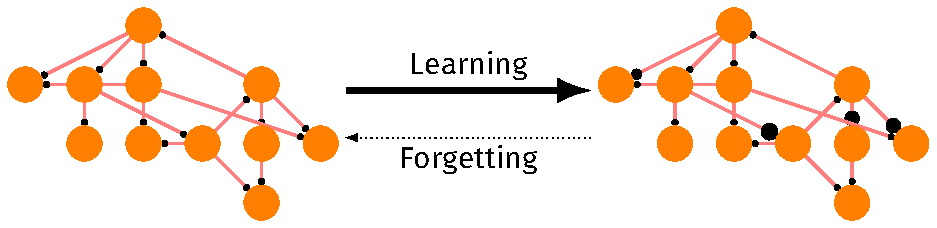
\includegraphics[width=\linewidth]{engram.pdf} 
\end{figure}

I can recall an experience as long as the set of synapses in which the
particular experience was stored remains \emph{intact}. Therefore, our ability
to remember is contingent on our brain's ability to keep its connections intact.
But on the other hand, our ability to learn depends on our brain's ability to
change its connections. And here is the first challenge!

\subsection{Learning quickly v/s forgetting slowly, a zero-sum game}\label{subsec:zero_sum} 
\leftHighlight{
    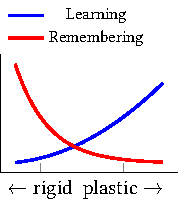
\includegraphics[]{./foget_remember.pdf}
    Ability to change (plasticity) is good for learning, but bad for remembering.
}

For $M_\text{Lalu}$ (or any other memory) to remain intact, each synapse which
participated in its formation (i.e., $s_{10}, s_{21}, s_{12} \ldots$) should
remain intact. The longer a synapse can keep itself unchanged, the better it
will be at keeping the memory safe. Let's assume that somehow I create a synapse
which maintains its state for a very long time (i.e., a rigid synapse). This
synapse will not \emph{forget} easily, but it will not participate in any new
memory formation either. Learning requires synapse to change and a rigid syanpse
can't change.  Rigid synapses behave like a read-only Compact Disk (CD). On the
other hand, if I create a synapse which is easily changeable (i.e., a plastic
synaspe), it will be good at learning new experiences but won't be able to
retain them for long. Plastic synapse forgets easily.  We know that we not only
remember for long time, we are also capable of learning quickly. And not just
us, many other animals are quick to learn. Honey bees can learn the location of
food after one encounter with food source such a flowers. Indeed, a good memory
system is the one which learns as quickly as possible from rewarding or painful
experiences and forgets as slowly as possible. Forgetting and remembering are
two sides of the same coin. They are conflicting demands i.e., improving one
will deteriorate the other -- a zero-sum game.  The challenge is to strike a
balance. 

% Hopfield network 
\section{Hopfield network -- associative memory network}\label{sec:hopfield}

Memory storage and retrieval is trivially done by a computer. It will be helpful
to compare memory storage in the computer and the brain. In the computer, we
always know the address of every stored memory and we access it by providing
this address. The file icon on your desktop is a graphical way of encoding this
addressing scheme. This process is similar to looking up the index page in a
reference book to find a topic. Our brain, on the other hand, is very unlikely
to have such an indexing mechanism. 

We recall when we are provided with \textit{cues}. For example, when you see
some part of a familiar person in a wedding album -- while the rest of the
person may be hidden behind others -- you could easily identify the person.
Many other memories of that person will also be recalled. A famous class of
recurrent neural network popularly known as Hopfield network can do just the
same as shown in \Fig{fig:hopfield}.

\begin{figure}[!hb]
    \centering
    \caption{Hopfield network with 100 spiking neurons. These \emph{recurrent} 
        configurations give rise to interesting brain-like
        computation. \textbf{(B)} 6 patterns (memory) i.e. NCBSXY are stored in this
        network. \textbf{(C)} When a very distorted \textit{cue} is applied to
        the network input, it \textit{fetches} one of stored pattern which is
        the \emph{closest} to the applied cue.
    }\label{fig:hopfield}
    \includegraphics[width=\linewidth]{./hopfield.pdf}
\end{figure}

How does this recurrent network work is beyond the scope of article. Readers are
encouraged to explore more by themselves. \emph{``How well can we explain
biological memory by these networks?''} is an active research area.  Though
these networks are extremely successful in accomplishing various
\textit{brain-like} computations (\textit{a la} machine learning), I would like
to advise the reader to be skeptical by noting the following:

\begin{itemize}
    \item  Neurons used in these networks are highly simplified. \textit{Real}
        neurons are not this simple. Even though these simplified neurons
        capture the essential \textit{all-or-none} (electrical spike) way of
        communication and learning by changing synaptic connections, they do
        ignore rich local computations which can be accomplished by branches of
        these neurons called \textit{dendrites}.
    \item  There is no evidence that neurons make such dense recurrent
        connections. However some studies have shown that Hopfield network can
        work with very sparse recurrent connections as well.
    \item Activity in these networks does not match usually observed activity 
        in the primate brain during memory-recall experiments.
\end{itemize}

\leftHighlight{Solutions contributed by other disciplines are helpful for
comparison and contrast and often provide very useful insight. But in the end, these
solutions must be tested under the constraints imposed by biology.}

Nonetheless, these networks provide us with a framework to concretely think
about the problem of memory storage and recall. We learn a great deal about a
problem by pointing out the limitations and failures of models which describe
it. Hopfield network has properties which will sound very natural to us. Can you
store as many memories as you like in these networks? No. There is an upper
limit. Adding more patterns over maximum limit causes distortion in memories.
When a cue is given, the network no longer fetches the right pattern. It often
fetches a pattern which was not even stored; the retrieved pattern instead
resemble some mixture of stored patterns. When too many memories are stored,
they corrupt each other by mixing up. One can ask more questions. When
connections decay in these networks and memories start disappearing, which
memory disappear first: the weakest or the newest? And, when a new memory
closely associated with an old memory is added, what happens to that old
memories?

After this necessary detour, lets go back to the main theme: how do synapses
maintain their state?

\section{How does a synapse maintain its state?}

Very complex biochemistry plays out during learning that changes the synapse.
Surprisingly, the net effect of this complex biochemistry can be summarised by a
simple mathematical expression. Ah, \emph{the unreasonable effectiveness of
mathematics}\cite{unreasonable_math}! Let's assume that synaptic strength $w$ is
tightly correlated with a chemical species $X$ found at synapse i.e. $w$ changes
with $X$. The problem of maintenance of $w$ can be rephrased as the problem of
maintenance of the activity of $X$. Therefore, the problem of ``\emph{synapse
maintaining its state}'' becomes the problem of ``\emph{molecule $X$ maintaining
its state}'' -- a more concretely defined problem.

Let's assume that $X$ is converted to its active form $X^*$  by adding a
\rightHighlight{ \raggedright 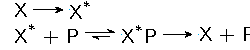
\includegraphics[width=3.5cm]{./fig_model.pdf} }
phosphoryl group ($PO_3^{2-}$). The phosphoryl group is removed by a phosphatase
and $X^*$ is turned back into inactive $X$. The phosphorylation and its
counterpart dephosphorylation are a very common motif for controlling various
chemical reactions by activating and inactivating protein molecules. Once most
$X$ has been turned into $X^*$ during memory formation, how do we make sure that
$X^*$ does not turn back into $X$ (lose memory)?

Let's mull over a solution to this problem of long term maintenance of $X^*$.
Here is one potential solution.

\begin{enumerate}
    \item \textbf{(Amplification)} $X^*$ \textbf{auto-phosphorylates} itself i.e. \tikz[baseline]{ 
            \node (x) {$X$};
            \node[right=9mm of x] (xp) {$X^*$};
            \draw[-latex] (x) -- (xp);
            \draw[-latex] (xp) edge[out=120, in=90] ([xshift=7mm]x);
        }. If we manage to get sufficient $X^*$ somehow, it
        will act as a catalyst to its own production. $X^*$ will always remain
        high.
    \item Dephosphorylation of $X^*$ is minimized by controlling the number of
        $P$ or reducing the reaction rate.
\end{enumerate} 
\rightHighlight{Can you think of other set of hypotheses? It must conform to
laws of chemistry!}

Both (1) and (2) help in making $X^*$ highly stable. Problem solved? No.  Now
we have constructed a rigid synapse. Recall the \textit{rigid} v/s
\textit{plastic} synpase dilemma discussed previously (section
\ref{subsec:zero_sum}). This synapse will definitely remember for longer
but it will not participate in any new learning anymore.

As long as we are in the realm of theory, let's propose a solution to this
problem. We add another reaction say $P'+X^*\rightarrow P'X \rightarrow P'+X$
which deactivates $X^*$ when the \textit{need} arises. Phosphatase P' is
different from P. This adds another layer of control to an already complicated
problem i.e.  forgetting is now controlled by another process. This requires one
more explanation: how does this new mechanism controlling \textit{forgetting}
work?  And philosophically -- if you care about it -- it violates the principle
of \textbf{parsimony} which recommends to pick the simplest explanation.

We still have two big problems hiding underneath. We have not considered the
underlying biological hardware i.e. synapse in any detail where this biochemical
network suppose to function. The first problem is chemical noise . For a
biochemical system operating in very small volumes, effect of chemical noise can
be very strong. \leftHighlight{The volume of a typical synapse is
\SI{1e-20}{\cubic\meter}. At this volume, \SI{1}{\micro M} concentration is
roughly equal to 6 molecules.} There are over 200 types of protein molecules in
a typical synapse. Indeed, most of these protein molecules have few tens of
molecules. The brain is always active and the chemical noise caused by the
brain's background activity will surely turn some molecules of $X$ into $X^*$.
Then due to auto-phosphorylation, sooner than later, all of the $X$ will be
turned into $X^*$. We have created a very stable memory of nothing but
background noise. This is highly undesirable!

The second problem is \textit{turnover} i.e. old molecules are continuously
degraded and being replaced by newly minted molecules. Let's assume that at the
time of memory formation, we had 100 molecules of $X^*$ in the synapse. And
let's also assume that on average, every day one new formed molecule (i.e. $X$)
replaces an old one ($X^*$).  After 50 days, half of the synaptic strength is
gone! To counter this, we must have a \textit{refresh} mechanism by which the
newly added molecule quickly changes its state according to the state of synapse
i.e. newborn $X$ becomes $X^*$ if most molecules at synapses are $X^*$.

\begin{figure}[b!]
\centering
\caption{A hypothetical network which can solve the problem of chemical noise and
    turnover with suitable parameters. The activation step is divided
    into slow and fast components such that fluctuations caused by background
    noise do not cause the system to activate itself. $X^*$ also partially activate
    $X$ to $X^\sim$ to overcome \textit{turnover.}
}\label{fig:model_bistable}
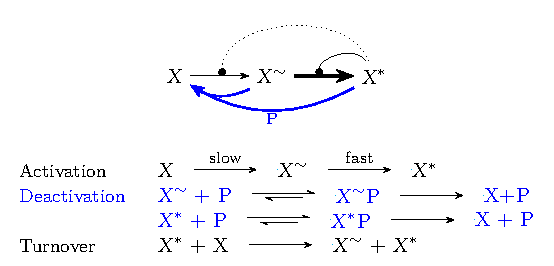
\includegraphics[width=\linewidth]{./fig_model_b.pdf}
\end{figure}

Effectively, we want a stable \texttt{ACTIVE} state (all $X$ are $X^*$) which is
immune to turnover. We also don't want chemical noise to turn $X$ into $X^*$.
We want a switch like behaviour i.e. if it is \texttt{OFF} or \texttt{ON} it
tends to stay \texttt{OFF} or \texttt{ON}. If a few $X$ are turned into $X^*$ by
background noise, we want them to be quickly turned back into $X$ by the
phosphatase $P$. And if during memory formation, a significant portion of $X$
has been turned into $X^*$ then we want that any $X^*$ deactivated into $X$ is
quickly activated again into $X^*$. This system should operate like a switch
which does not flip unless significant force is applied. These are called
\textbf{bistable switch}es (See Box 1 for overview of bistability). 

Is there any evidence that bistable chemical reaction networks exist? Do they
occur at all in living cells?  Bistability (and its close relative oscillations)
are very common in biology (What is the reason for their \emph{selection}
by evolution?); from cellular level to population levels. So it
won't be surprising if we discover bistable switches operating at syanpse as
well. Indeed, various studies have shown that \gls{camkii} \emph{may} form a
bistable switch in synapse.

\section{Molecular bistable switch at synapse}\label{sec:molecular_switch}
\rightHighlight{
    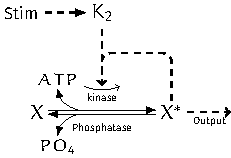
\includegraphics[width=4cm]{./lisman_bistable_small.pdf}
    Reaction in a bistable switch proposed by John Lisman. Modified
    from \cite{lisman1985}. 
    \label{fig:lisman}
}

Late John Lisman hypothesised that a kinase and a phosphatase together can form
a bistable switch immune to \emph{turnover}. \gls{camkii} and its phosphatase
\Gls{pp1} were identified as the hypothesised kinase and phosphatase. This
chemical system has been extensively studied using computational models for over
two decades \cite{sandstorm}. There is some evidence that \gls{camkii} is
bistable \emph{in vitro} conditions. Whether \gls{camkii} is bistable inside a
living neuron is still an open question (see Box 2 for overview of \gls{camkii}
properties at synapse.).

% Bistable box
\boxTexteven{Bistability in reaction network} {
    \def\StateA{\tikz \node[circle, dashed, draw, inner sep=1pt] {\scriptsize
    \textsf{A}};}
    \def\StateB{\tikz \node[circle, dashed, draw, inner sep=1pt] {\scriptsize
    \textsf{B}};}

    In a world full of fluctuations, stability is indeed very useful property.
    Life is remarkably stable even though it is made up of inherently noisy
    components. Bistable chemical networks are ubiquitous in biology. In
    bistable chemical networks, noisy components acts together to give rise to 
    highly (bi)stable behaviour. \emph{Also note that even though the underlying
    reactions are almost always reversible, the bistable switch is usually not
    reversible.} Isn't it a neat way for taking decisions?

    A bistable system -- as its name implies -- has two stable states. From the
    point of view of an experimentalist, if you obverse a bistable system for
    very long time, you would almost always find it in either of its two stable
    states. Just like an electrical switch which you would almost always find in
    either \texttt{ON} or \texttt{OFF} state (and rarely in transition between
    states).

    \vspace{3mm} 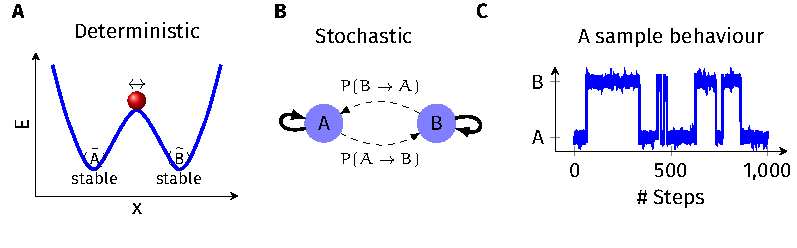
\includegraphics[width=\linewidth]{./stability_noise.pdf} 

    In the figure above, \textbf{A} show a conceptual model of bistability.  The
    energy landscape of a bistable system has two minima (\StateA and \StateB),
    therefore, the system always ends up in either of them. It is a
    deterministic bistable system. \textbf{B} shows a conceptual representation
    of stochastic bistable system as state transition diagram.  The arrows
    depict the probability of transition from one state to the other. In
    \textbf{C}, we simulate the system described in \textbf{B} with probability
    of transition from A to B ($P(A\rightarrow B)$), and from B to A
    ($P(B\rightarrow A)$) set equal to 0.01. 

    Such bistable motif are commonplace in biology \cite{ramakrishnan2008},
    especially found in situations where cell has to make a decision. One such
    motif is show below in both deterministic and stochastic settings. There are
    three necessary conditions a network must have to be able to show
    bistability: positive feedback, mechanism to filter out small stimuli, and a
    mechanism to prevent explosions\cite{wilhelm}. 

    \vspace{3mm}
    \begin{tikzpicture}[scale=1 , every node/.style={} ]
        \node[] (img) {
                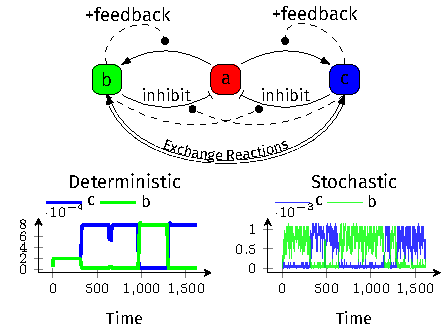
\includegraphics[width=6.5cm]{./strong_bis_naren_and_bhalla_87mm.pdf}
            };

        \node[right=0mm of img, text width=6cm, align=justify] {
                A bistable chemical system adapted from \cite{ramakrishnan2008}.
                Species \texttt{b} and \texttt{c} catalyze their production
                (positive feedback) and inhibits production of \texttt{a}.
                \textbf{(below)} Two trajectories are shown in different
                settings. (Left) System is deterministic; (right) System is stochastic.
            };
    \end{tikzpicture}	
}

% CaMKII box.
\boxTextodd{\gls{camkii} at synapse: A brief overview of its properties and function} {
    Among more than 2000 proteins found in brain, \gls{camkii} constitutes roughly
    2\% of them all. Furthermore, it is enriched in the hippocampus -- a brain structure
    necessary for memory formation. Indeed, \gls{camkii} is known to play essential
    role in learning and memory. In experiments involving mice, deactivating
    \gls{camkii} in any way has always resulted in impairment of memory formation
    and learning. 

    \gls{camkii} molecule has interesting properties which makes it an
    attractive candidate for storing information. 12 or 14 subunits of
    \gls{camkii} make up one holoenzyme, usually arranged in dodecameric (top
    view \tikz{  \foreach \i in {1,2,...,6} { \node[circle, fill=blue!50,
            shift=(60*\i:1mm),inner sep=1pt] (b\i) at (0,0) {}; } }) or
            tetradecameric form (top view \tikz{ \foreach \i in {1,2,...,7} {
            \node[circle, fill=blue!50, shift=(360*\i/7:1mm),inner sep=1pt]
    (b\i) at (0,0) {}; } }). \gls{camkii} structure is shown in (\textbf{A})
    inset below (from Protein Data Bank (https://www.rcbs.org)).

    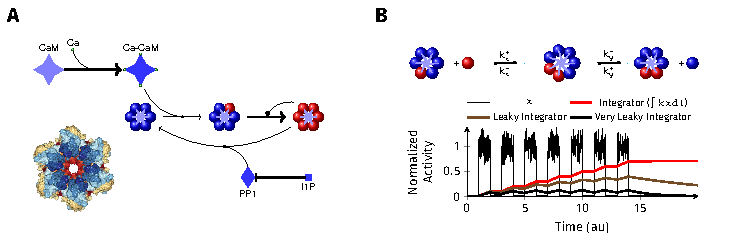
\includegraphics[width=13cm]{./camkii_properties.pdf}

    \textbf{(A)} Summary of \gls{camkii} pathway of. Upon its influx into
    synapse, \gls{ca} binds to \gls{cam} and create a complex \gls{cacam}.
    \gls{cacam} binds to \gls{camkii} and phosphorylate it.  \gls{camkii} is
    dephosphorylated by \gls{pp1}. \textbf{(B)} Subunit exchange
    between two holoenzymes i.e. a fully active \gls{camkii} holoenzyme can
    loose an \textit{ACTIVE} subunit which can be picked up by another
    holoenzyme which becomes partially active. 
    
    First step of \gls{camkii} activation is very slow for it requires binding
    of two \gls{cacam} simultaneously. Once a subunit has been activated (red
    circle), phosphorylation of its neighbours requires binding of only one
    \gls{cacam} and therefore further phosphorylation proceeds at much faster
    rate.  Note that the first very slow step can be overcome by subunit
    exchange when an inactive holoenzyme picks up an active subunit released by
    other holoenzyme. Therefore subunit exchange helps in spreading \gls{camkii}
    activation. 

    \textbf{\gls{camkii} integrates \gls{ca} signal} A single \gls{camkii}
    holoenzyme acts as a leaky integrator of \gls{ca} activity i.e. it sums up
    \gls{ca} activity in time and also decays with a time-constant (leaky). See
    \textbf{(B)} to compare behaviour of three integrators of calcium activity
    ($x$): a non-leaky integrator and two leaky integrators with small and large
    amount of leakage.  Mathematically, it is similar to a leaky capacitor if we
    model \gls{ca} activity as applied current and \gls{camkii} activity as
    voltage across capacitor.  Integrators are useful when you want to
    accumulate \emph{enough} information about $x$ before taking a decision e.g.
    a plant can \emph{decide} to flower or shed leaves only if integration of
    moisture in air and/or temperature during the day crosses a threshold value.

} % box

In our computational study of this pathway, we explored the effect of subunit
exchange on \gls{camkii} pathway \cite{SinghAndBhalla2018}.  We found that the
subunit exchange improves information retention capacity of \gls{camkii}. This
adds weightage to the idea that \gls{camkii} is \textit{the memory melecule}.
Individual \gls{camkii} acts as leaky integrator of \gls{ca} activity (see Box
2.). With subunit exchange, the leaky integrator becomes less leaky and hold
information for longer time. When many \gls{camkii} holoenzymes come together
and form a cluster then they give rise to a bistable switch
(\Fig{fig:camkii_sync}). Such clusters have been observed in experiments. We
found that subunit exchange synchronizes bistable activity of distributed
clusters.  That is multiple bistable switches act as a single but much more
stable bistable switch. To summarise, we found the subunit-exchange makes
\gls{camkii} molecule better at retaining information.

\begin{figure*}[t!]
    \caption{ \textbf{(A)} (left) Three clusters of \gls{camkii} in a synapse
        . (Right) This system ability to hold memories increases exponentially
        with system size. 52 holoenzymes can keep the memory intact roughly for
        100 years! \textbf{(B)} Subunit exchange improves \gls{camkii} ability
        to store information. \textbf{(Red)} 3 individual bistable switches independently  
        without subunit exchange. \textbf{(Blue}) When subunit exchange is enabled, these 
        independent switches synchronize. Notice that the now system spends more 
        time in its stable states.
    }\label{fig:camkii_sync}
    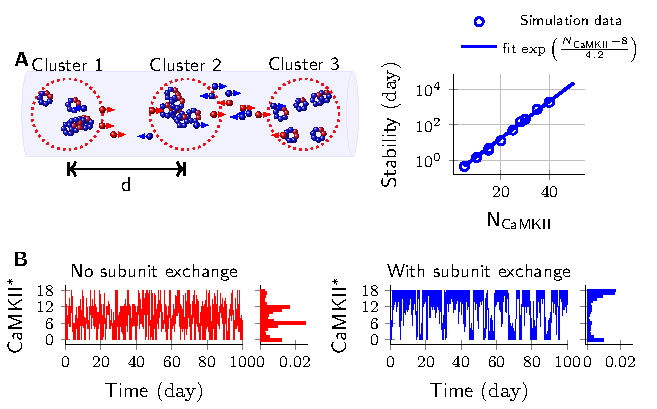
\includegraphics[width=\linewidth]{./bistable/Fig5/figure_sync_114mm.pdf}
\end{figure*}


% References section
\section{Conclusion}

In this article, we have discussed why bistable motif is an attractive candidate
for storing biological memories. They are ubiquitous in biology and are natural
solution to the problem of memory maintenance under chemical noise and turnover.
We have also discussed a potential pathways (\gls{camkii}) which may be bistable
at synapse. Now let's put all of this to a reality check. Let's assume that
bistables mechanism exists at synapse. We know that size of a synapse is tightly
correlated with its strength. That means we can observe synapse size as the
proxy of its strength. If we observe synapse for long time and record its size
continuously, what would we observe? If the distribution of size is bimodal (two
peaks) than its a strong suggestion that underlying mechanism is bistable. More
strongly, if the underlying mechanism is bistable, then I \emph{must} observe a
bimodal distribution.

There is now growing experimental evidence that synaptic size change in
\textit{all-or-none} manner, a finding which is consistent with this idea. Some
other studies have claimed that changes are graded i.e. synapse changes in
step-wise manner much like a \textbf{multi-stable} synapse. A multi-stable
synapse is an additive ensemble of many bistable components
(\Fig{fig:fig_bistable_multistable}).

\begin{figure}[ht!]
    \centering
    \caption{\textit{All-or-note} v/s graded synapse and mechanism which may
        give rise to them. \textbf{(A)} A bistable mechanism (red) controlling the 
        synaptic strength.  Synapse size changes in \textit{all-or-none}
        fashion. \textbf{(B)} A multi-stable mechanism (red) gives rise to a graded synapse (blue) 
        which changes its size in step-wise manner. Note that a multi-stable
        mechanism can be constructed by adding multiple bistable switches (4
        bistable switches shown in light blue in blue are used in this case).
    }
    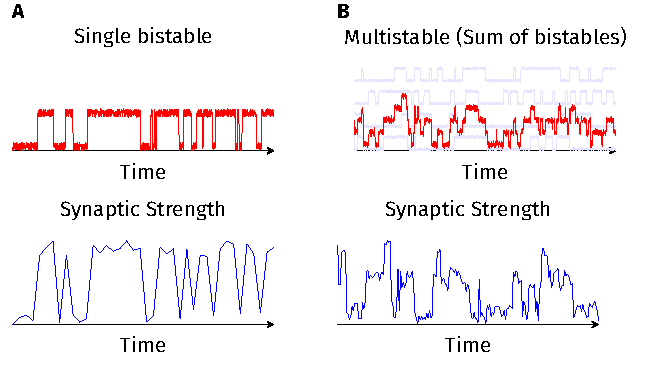
\includegraphics[width=\linewidth]{./bistable_multistabe_synapse.pdf}
    \label{fig:fig_bistable_multistable}
\end{figure}

Whether \gls{camkii} is bistable in the synapse is still an open question.
Neither there is any concrete evidence that it is nor it has been ruled out that
it is not, especially near the membrane. Our aim in this article was to argue
why bistable mechanism is a good solution to the problem of storing memory for
long time. Even if \gls{camkii} turns out to be not bistable at synapse, there
could be other unknown mechanisms which can give rise to bistability. Given that
bistable chemical motifs are widespread, it is reasonable to suggest that there
are indeed switches in our brain -- much like flip-flops in the digital memory
card of your phone -- which are evolved to keep our memories safe from the
onslaught of time and noise.

\section*{Acknowledgements} I'd like to thank Somya Mani and Bhanu Priya for
helpful suggestions on the manuscript.

\correspond{
    Bhalla Lab,
    National Center for Biological Sciences, Bengaluru \\
    GKVK Campus, Bellary Road \\
    Bengaluru - 560065.  \\
    Email: dilawars@ncbs.res.in
}

\begin{thebibliography}{99} 
    \bibitem{lisman1985} 
    Lisman J. E., 
    \textit{A mechanism for memory storage insensitive to molecular turnover: a
    bistable autophosphorylating kinase}. 
    Proc. Natl. Acad. Sci. USA, May 1985

    \bibitem{koch1999}
    Christof Koch
    \textit{Biophysics of computations}.
    Oxford University Press, 1999

    \bibitem{sandstorm} 
    Malin Sandstorm,
    \textit{Models of CaMKII activation},
    Master Thesis, Royal Institute Of Technology Sweden 

    \bibitem{unreasonable_math}
    Eugene Wigner,
    \textit{The Unreasonable Effectiveness of Mathematics in the Natural Sciences},
     Communications in Pure and Applied Mathematics, vol. 13, No. I (February 1960)

    \bibitem{wilhelm}
    Thoman Wilhelm,
    \textit{The smallest chemical reaction system with bistability},
    BMC Systems Biology, vol. 3, No 1 (Sep 2009)

    \bibitem{ramakrishnan2008}
    Naren Ramakrishnan, Upinder S. Bhalla
    \textit{Memory Switches in Chemical Reaction Space},
    PLOS Computational Biology, No 7 vol. 4 (July 2008)

    \bibitem{SinghAndBhalla2018}
    Dilawar Singh, Upinder S Bhalla,
    \textit{Subunit exchange enhances information retention by CaMKII in dendritic spines},
    biorxiv, doi:10.1101/372748 (2018)

    \bibitem{stratton}
    Stratton M et al.,
    \textit{Activation-triggered subunit exchange between CaMKII holoenzymes
    facilitates the spread of kinase activity}, Elife (Jan 2014) 

\end{thebibliography}

\end{document}
